\documentclass[12pt,a4paper]{article}
\usepackage[utf8]{inputenc}
\usepackage[english,russian]{babel}
\usepackage{hyperref}
\hypersetup{
	colorlinks   = true, 
	urlcolor     = blue, 
	linkcolor    = blue, 
	citecolor   = red
}
\usepackage{amsthm,amssymb,amsfonts,amsmath}
\usepackage{physics}
\usepackage{xcolor}
\usepackage{svg}
\usepackage[left=3cm,right=3cm,
top=3cm,bottom=3cm,bindingoffset=0cm]{geometry}
\usepackage{tcolorbox}
\usepackage{physics}
\tcbuselibrary{theorems}

\newtcbtheorem
[number within=section, 
list inside={def}]
{definition}
{Определение}
{
	colback=red!3,
	colframe=red!20!white,
	coltitle=black,
	fonttitle=\bfseries,
	sharp corners,
}
{def}

\tcbuselibrary{theorems}
\newtcbtheorem
[number within=section]
{proposition}
{Утверждение}
{
	colback=purple!3,
	colframe=purple!25!white,
	coltitle=black,
	fonttitle=\bfseries,
}
{prop}

\tcbuselibrary{theorems}
\newtcbtheorem
[number within=section]
{theorem}
{Теорема}
{
	colback=blue!3,
	colframe=blue!20!white,
	coltitle=black,
	fonttitle=\bfseries,
}
{th}

\tcbuselibrary{theorems}
\newtcbtheorem
[number within=section]
{example}
{Пример}
{
	colback=orange!3,
	colframe=orange!20!white,
	coltitle=black,
	fonttitle=\bfseries,
	sharp corners,
}
{exmpl}

\tcbuselibrary{theorems}
\newtcbtheorem
[number within=section]
{lemma}
{Лемма}
{
	colback=gray!3,
	colframe=gray!20!white,
	coltitle=black,
	fonttitle=\bfseries,
}
{lemm}

% Непрерывное вложение
\makeatletter
\newcommand{\rightarrowhead}{\mathrel{%
		\hbox{\let\f@size\sf@size\usefont{U}{lasy}{m}{n}\symbol{41}}}}

\newcommand\arrsubset{\mathrel{\ooalign{$\subset$\cr
			\hidewidth\raise-0.440ex\hbox{$\rightarrowhead\mkern0.5mu$}}}}
% Непрерывное вложение

% Для удобства
\newcommand{\intset}[1]{\int\limits_{#1}}
\newcommand{\Real}{\mathbb{R}}
\newcommand{\Natural}{\mathbb{N}}
\newcommand{\ssubset}{\subset \subset}
\newcommand{\Dto}{\overset{\mathcal{D}}{\to}}
\newcommand{\nnorm}[1]{{\left\vert\kern-0.25ex\left\vert\kern-0.25ex\left\vert #1 
		\right\vert\kern-0.25ex\right\vert\kern-0.25ex\right\vert}}
\DeclareMathOperator\supp{supp}
\DeclareMathOperator\dist{dist}
\DeclareMathOperator\diam{diam}
\DeclareMathOperator{\bounded}{B}

\date{}
\title{Соболевские пространства}
\author{Самутичев Е.Р.}

\begin{document}
	
\maketitle
\begin{abstract}
	Собраны основные понятия и утверждения курса лекций, читаемых С.В. Лупуляком в СПбПУ. Крайне избирательно присутствуют доказательства. Конспект удобно использовать как справочник, в конце есть список определений. 
\end{abstract}

\section{Усреднение функций}
	
\subsection{Основные понятия}

Пусть в $\Real^n$ задана норма 
$$|x| = \sqrt{\sum_{i=1}^{n}{x_i^2}}$$ 
Определим $\omega: \Real^n \to \Real$ как
\begin{equation*}
	\omega (x) = 
		\begin{cases}
		c e^{\frac{1}{|x|^2 - 1}}, & x \in B(0, 1) \\
		0, & x \notin B(0, 1)
		\end{cases}
\end{equation*}
где 
$$c  = \frac{1}{\intset{B(0,1)}{e^{\frac{1}{|x|^2 - 1}}dx}}$$
так что $\intset{B(0,1)}{\omega(x)dx} = 1$ и кроме того по определению $\omega \in C(\Real^n)$. \\ Пусть $\omega_\rho (x) = \rho^{-n} \omega \left(\frac{x}{\rho}\right)$, тогда свойства указанные выше сохраняются.

\begin{definition}{Усреднение функции}{def:1}
	Пусть $\rho > 0$, усреднением функции $u \in L^{1}(\Omega)$ называется 
	$$u_\rho (x) = \intset{\Omega}{\omega_\rho (x - y) u(y) dy}, \forall x \in \Real^n$$
	Важное свойство $u_\rho \in C^{\infty}(\Real^n), \forall \rho > 0$
\end{definition}

\begin{proposition}{Вложенность $L^p$}{prop:1}
	Пусть $\Omega \subset \Real^n$ -- открытое ограниченное, тогда
	\begin{enumerate}
		\item $L^{\infty}(\Omega) \subset \underset{1 < p < \infty}{L^{p}(\Omega)} \subset L^{1}(\Omega)$
		\item $L^{p}(\Omega) \subset L^{q}(\Omega), 1 \leq q < p \leq \infty$
	\end{enumerate}
\end{proposition}

\begin{proposition}{О норме усреднения}{prop:2}
	Пусть $u \in L^{p}(\Omega), 1 \leq p \leq \infty$, тогда 
	$$\norm{u_\rho}_{L^{p}(\Omega)} \leq \norm{u}_{L^{p}(\Omega)}$$
\end{proposition}

\begin{proposition}{О сходимости усреднений в $C$}{prop:3}
	Пусть $u \in C(\Omega)$, $\underset{\text{компакт}}{K} \subset \Omega$, тогда $u_\rho \underset{\rho \to 0}{\to} u$ в $C(K)$
\end{proposition}
Из последнего утверждения следует что $u_\rho (x) \underset{\rho \to 0}{\to} u (x), \forall x \in \Omega$.

\begin{theorem}{О сходимости усреднений в $L^{p}$}{th:1}
	Пусть $u \in L^{p}(\Omega), 1 \leq p < \infty$, тогда $u_\rho \underset{\rho \to 0}{\to} u$ в $L^{p} (\Omega)$
\end{theorem}

\subsection{Свойства функций из $L^p$ связанные с усреднением}

Рассмотрим множества плотные в пространствах Лебега.
\begin{proposition}{}{prop:4}
	$C^{\infty} (\overline{\Omega})$ плотно в $L^p (\Omega), 1 \leq p < \infty$
\end{proposition}

\begin{proposition}{}{prop:5}
	$C^{\infty}_0 (\Omega)$ плотно в $L^p (\Omega), 1 \leq p < \infty$
\end{proposition}

\begin{definition}{Вхождение с замыканием}{def:2}
	$\Omega^{'} \ssubset \Omega$ если $\Omega^{'}$ -- предкомпакт и $\overline{\Omega^{'}} \subset \Omega$
\end{definition}

\begin{definition}{Локально суммируемые функции}{def:3}
	$u \in L^{p}_{\text{loc}} (\Omega)$ -- $u$ локально суммируема с показателем $p$, если \\ $u \in L^{p} (\Omega^{'}), \forall \Omega^{'} \ssubset \Omega$
\end{definition}
Заметим что на ограниченной области локально суммируемые функции ведут себя как угодно на границе.

\begin{example}{}{exmpl:1}
	$f \equiv c$, $f \notin L^1 (\Real)$, но $f \in L^1_{\text{loc}} (\Real)$
\end{example}

\begin{lemma}{Дюбуа-Реймонда}{}
	Пусть $u \in L^1_{\text{loc}} (\Omega)$ и $\intset{\Omega}{u\varphi dx}, \forall \varphi \in C^{\infty}_0 (\Omega)$, тогда $u = 0$ п.в. на $\Omega$ [Заметим что класс для $u$ очень широкий, а для $\varphi$ очень узкий]
\end{lemma}

\subsection{Критерий компактности в $L^p$}

Пусть $\Omega$ -- ограниченная область, $F \subset L^p (\Omega), 1 \leq p < \infty$, по умолчанию $f \in F$ продолжаем 0 на $\Real^n$
\begin{theorem}{Критерий Рисса}{th:2}
	$\underset{\text{предкомпакт}}{F} \subset L^p (\Omega) \Leftrightarrow$
	\begin{enumerate}
		\item $\exists M \geq 0: \norm{f}_{L^p (\Omega)} \leq M, \forall f \in F$
		\item $\sup\limits_{f\in F}{\sup\limits_{|z| < \rho}{\norm{f(x+z) - f(x)}_{L^p (\Omega)}}} = \delta(\rho) \to 0$
	\end{enumerate}
\end{theorem}

\section{Обобщенные функции}

\subsection{Мотивация}

Пусть $f \in C^1 (\Omega), \varphi \in C_0^\infty (\Omega)$, тогда
\begin{equation*}
	\intset{\Omega}{\frac{\partial f}{\partial x_i} \varphi dx} \overset{\text{по частям}}{=} \intset{\partial \Omega}{f \varphi n_i d\sigma} - \intset{\Omega}{u \frac{\partial \varphi}{\partial x_i} dx} \overset{\varphi \equiv 0 \text{ вне } \Omega}{=} 0 - \intset{\Omega}{u \frac{\partial \varphi}{\partial x_i} dx} = -\intset{\Omega}{u \frac{\partial \varphi}{\partial x_i} dx}
\end{equation*}
или
\begin{equation*}
	\intset{\Omega}{f^\prime \varphi dx} = -\intset{\Omega}{f \varphi^\prime dx}
\end{equation*}
функцию $f^\prime$ удовлетворяющую этим свойствам можно найти для более широкого класса функций.

\subsection{Пространства основных функций}

\begin{definition}{D-сходимость}{def:4}
	Пусть $\Omega \subset \Real^n$ -- открытое, в $C_0^\infty (\Omega)$ определим сходимость (именуемую D-сходимостью) как:
	$\varphi_m \Dto \varphi \Leftrightarrow$
	\begin{enumerate}
		\item $\exists \underset{\text{компакт}}{K} \subset \Omega: \supp \varphi \subset K, \ \supp \varphi_m \subset K$
		\item $D^\alpha \varphi_m \to D^\alpha \varphi \text{ в } C(K), \forall \alpha \text { -- мультииндекса}$
	\end{enumerate}
\end{definition}

\begin{definition}{Пространство основных фунцкий}{def:5}
	$C_0^\infty (\Omega)$ в совокупности с D-сходимостью образует $D(\Omega)$ -- пространство основных функций
\end{definition}

\begin{definition}{Распределение}{def:6}
	Распределением или обобщенной функцией называется линейный функционал $T : D(\Omega) \to \Real$ непрерывный относительно D-сходимости, т.е. такой что:
	\begin{enumerate}
		\item $T(\alpha_1 \varphi_1 + \alpha_2 \varphi_2) = \alpha_1 T(\varphi_1) + \alpha_2 T(\varphi_2), \forall \alpha_1, \alpha_2 \in \Real, \ \forall \varphi_1, \varphi_2 \in D(\Omega)$
		\item $\varphi_m \Dto \varphi \Rightarrow T(\varphi_m) \to T(\varphi)$
	\end{enumerate}
	Множество распределений обозначают как $D^* (\Omega)$
\end{definition}

\begin{proposition}{}{prop:6}
	$D^* (\Omega)$ -- линейное многообразие
\end{proposition}

\begin{example}{Регулярные распределения}{exmpl:2}
	Пусть $f \in L_{\text{loc}}^1 (\Omega)$, определим $T_f (\varphi) = \intset{\Omega}{f \varphi dx}, \forall \varphi \in D(\Omega)$. Можно показать что $T_f \in D^* (\Omega)$, распределения представимые таким образом называют регулярными. Остальные сингулярные.
\end{example}

\begin{example}{$\delta$-функция Дирака}{exmpl:3}
	Считая что $0 \in \Omega$ определим $T_\delta (\varphi) = \varphi(0)$. Можно показать что \\ $T_\delta \in D^* (\Omega)$ и это распределение не является регулярным т.е. сингулярно.
\end{example}

\begin{example}{Ограниченная мера Радона}{exmpl:4}
	Пусть $T \in D^* (\Omega)$ и $\exists M > 0: |T(\varphi)| \leq M \norm{\varphi}_{C(K)}$, где $K$ -- компакт такой что $\supp \varphi \subset K \subset \Omega$. Такое распределение называется ограниченной мерой Радона.
\end{example}

\subsection{Дифференцирование распределений}

\begin{definition}{Производная распределения}{def:7}
	$S = (-1)^{|\alpha|} (T \circ D^\alpha)$ -- это распределение (согласно следующему утверждению) называется частной производной распределения $T$, обозначается как $S = D^\alpha T$
\end{definition}

\begin{proposition}{}{prop:7}
	$D^\alpha T \in D^* (\Omega)$
\end{proposition}
Любое распределение таким образом дифференцируемо любое число раз.

\begin{example}{}{exmpl:5}
	Пусть $\Omega = \Real$ и $\chi(x) = 
	\begin{cases}
		1, &x \geq 0 \\
		0, &x < 0
	\end{cases}$, тогда 
	\begin{multline*}
		\frac{d}{dx}T_{\chi} (\varphi) = -T_{\chi}\left(\frac{d\varphi}{dx}\right) = -\int\limits_{-\infty}^{+\infty}{\chi \frac{d\varphi}{dx} dx} = -\int\limits_{0}^{+\infty}{\frac{d\varphi}{dx} dx} = -\lim_{M\to +\infty}{\int\limits_{0}^{M}{\frac{d\varphi}{dx}}} = \\ =\lim_{M\to +\infty}{\varphi(M) - \varphi(0)} = \varphi(0) - \lim_{M\to +\infty}{\varphi(M)} \overset{\text{финитность } \varphi}{=} \varphi(0) = T_\delta (\varphi)
	\end{multline*}
	т.е. $\frac{d}{dx}T_\chi = T_\delta$
\end{example}

\subsection{Обобщенные производные в смысле Соболева}

\begin{definition}{Обобщенная производная}{def:8}
	Пусть $\underset{\text{открытое}}{\Omega} \subset \Real^n, f \in L_{\text{loc}}^1 (\Omega)$ и $D^\alpha T_f$ -- регулярное распределение т.е. $\exists g \in L_{\text{loc}}^1 (\Omega): D^\alpha T_f (\varphi) = \intset{\Omega}{g \varphi dx}$, тогда $g$ называется обобщенной производной в смысле Соболева от $f$, это обозначается как $g = D_c^\alpha f$
\end{definition}
Нетрудно показать что если $f \in C^{|\alpha|} (\overline{\Omega})$, то $D_c^\alpha f = D^\alpha f$, т.е. это действительно обобщение понятия производной.

\begin{theorem}{О свойствах обобщенных производных}{th:2}
	Будем говорить что $u_m \to u$ в $L_{\text{loc}}^1 (\Omega)$ если $\forall \underset{\text{компакт}}{K} \subset \Omega: u_m \to u \text{ в } L^1 (\Omega)$. 
	\begin{enumerate}
		\item $u \in L_{\text{loc}}^1 (\Omega)$ и $\exists D_c^\alpha u$ в $\Omega$, тогда для $\Omega^\prime \subset \Omega$: $\exists D_c^\alpha (u|_{\Omega^\prime}) \text{ в } \Omega^\prime$ и \\ $D_c^\alpha (u|_{\Omega^\prime}) = (D_c^\alpha u)|_{\Omega^\prime}$
		\item $u_1, u_2 \in L_{\text{loc}}^1 (\Omega), c_1, c_2 \in \Real$ и $\exists D_c^\alpha u_1, D_c^\alpha u_2$ в $\Omega$, тогда \\ $\exists D_c^\alpha (c_1 u_1 + c_2 u_2) = c_1 D_c^\alpha u_1 + c_2 D_c^\alpha u_2$
		\item $\begin{cases} 
				D_c^\alpha u_m \to v &\text{ в } L_{\text{loc}}^1 (\Omega) \\
				u_m \to u &\text{ в } L_{\text{loc}}^1 (\Omega) 
				\end{cases}$, тогда $\exists D_c^\alpha u = v$
	\end{enumerate}
	Свойство 3 называется признаком обобщенной производной
\end{theorem}

\subsection{Усреднение функций имеющих обобщенные производные}

\begin{lemma}{}{}
	Пусть $u \in L^1 (\Omega)$ и $\exists D_c^\alpha u \in L_{\text{loc}}^1 (\Omega)$, $x\in \Omega: 0 < \rho < \dist(x, \partial \Omega)$, тогда $(D_c^\alpha u)_\rho (x) = (D^\alpha u_\rho) (x)$
\end{lemma}
Условие на $\rho$ существенно, в этом случае $\overline{B}(x, \rho) \subset \Omega$ т.е. $\omega_\rho (x - y)$ финитна по $y$ в $\Omega$.

\begin{lemma}{}{}
	Пусть $u \in L^p (\Omega), 1 \leq p < \infty$ и $\exists D_c^\alpha \in L^p (\Omega)$, тогда $\forall \Omega^\prime \ssubset \Omega: 
	\begin{cases} 
		u_\rho \to u &\text{ в } L^p (\Omega^\prime) \\ 
		D^\alpha (u_\rho) \to D_c^\alpha u &\text{ в } L^p (\Omega^\prime)
	\end{cases}$
\end{lemma}

\begin{lemma}{}{}
	Пусть $u \in L_{\text{loc}}^1 (\Omega)$ и $D_c^\alpha = 0 \text{ в } \Omega, \forall \alpha: |\alpha| = 1$ (все обобщенные производные 1-го порядка равны 0), тогда $u = const$ п.в. в $\Omega$
\end{lemma}

\begin{theorem}{Обобщенная производная в новых координатах}{th:3}
	Пусть $\Omega^\prime, \Omega \subset \Real^n, \varphi: \Omega^\prime \to \Omega$ -- диффеоморфизм, $u \in L_{\text{loc}}^1 (\Omega)$ и $\exists \frac{\partial_c u}{\partial x_i} \in L_{\text{loc}}^1 (\Omega), \forall i \in {1, ..., n}$, тогда $v = u \circ \varphi \in L_{\text{loc}}^1 (\Omega^\prime)$ и
	\begin{enumerate}
		\item $\exists \frac{\partial_c v}{\partial y_i} \in L_{\text{loc}}^1 (\Omega^\prime)$
		\item $\frac{\partial_c v}{\partial y_i} = \sum\limits_{k=1}^{n}{(\frac{\partial_c u}{\partial x_k} \circ \varphi)\frac{\partial \varphi}{\partial y_i}}$
	\end{enumerate}
\end{theorem}

\subsection{Случай одной независимой переменной}

\begin{definition}{Абсолютная непрерывность}{def:9}
	Функция $u: [a, b] \to \Real$ называется абсолютно непрерывной если \\ $\exists v \in L^1 ([a, b]): u(x) = \int\limits_a^x{v(t)dt} + u(a)$
\end{definition}
Можно доказать что абсолютно непрерывная функция равномерно непрерывна.

\begin{theorem}{Критерий существования обобщенной производной}{th:4}
	Для того чтобы $u \in L_{\text{loc}}^1 ([a, b])$ имела 1-ую обобщенную производную $\frac{d_c u}{dx} \in L^1 ([a, b])$ необходимо и достаточно чтобы она была абсолютно непрерывной.
\end{theorem}
\textbf{Мораль:} если $u$ -- суммируема и имеет суммируемую обобщенную производную, то она непрерывна.

\subsection{Пространства Соболева}

\begin{definition}{Пространства $W_p^\ell (\Omega)$}{def:10}
	Пусть $\underset{\text{открыт. огр.}}{\Omega} \subset \Real^n, 1 \leq p \leq \infty, \ell = 0, 1, 2, ...$, тогда определим пространства Соболева
	\begin{equation*}
	 	W_p^\ell (\Omega) = \{f \in L^p (\Omega) \ | \ \exists D_c^\alpha f \in L^p (\Omega), \forall \alpha: |\alpha| \leq \ell\}
	\end{equation*}
	Введем норму
	\begin{equation*}
		\norm{u}_{W_p^\ell (\Omega)} = \norm{u}_{p, \ell, \Omega} = \left( \intset{\Omega}{\sum\limits_{|\alpha| \leq \ell}{|D_c^\alpha u|^p}} \right)^{\frac{1}{p}}
	\end{equation*}
\end{definition}
Можно ввести и другую норму $\nnorm{u}_{p, \ell, \Omega} = \sum\limits_{|\alpha| \leq \ell}{\norm{D_c^\alpha u}_{L^p (\Omega)}}$

\begin{theorem}{}{th:5}
	$\left(W_p^\ell (\Omega), \norm{\cdot}_{p, \ell, \Omega}\right)$ -- банахово
\end{theorem}

\begin{proposition}{}{prop:7}
	$\norm{u}_{p, \ell, \Omega} \sim \nnorm{u}_{p, \ell, \Omega}$
\end{proposition}

\begin{definition}{Пространства $[L^p (\Omega)]^N$}{def:11}
	Определим пространства вектор-функций Лебега
	\begin{equation*}
		[L^p (\Omega)]^N = \{(u_1, ..., u_N) = \underline{u} \ | \ u_1, ..., u_N \in L^p (\Omega)\} 
	\end{equation*}
	Введем норму
	\begin{equation*}
		\norm{\underline{u}}_{[L^p (\Omega)]^N} = \left(\sum\limits_{i=1}^{N}{\intset{\Omega}{|u_i|^p dx}}\right)^{\frac{1}{p}}
	\end{equation*}
\end{definition}
Зачем вводятся эти пространства? На самом деле между $W_p^\ell (\Omega)$ и некоторым подпространством $[L^p (\Omega)]^N$, где $N = \sum\limits_{|\alpha| \leq \ell}{1}$ существует изометрический изоморфизм определяемый как $p: W_p^\ell (\Omega) \to [L^p (\Omega)]^N, p(u) = (D_c^\alpha u)_{|\alpha| \leq \ell}$ при лексикографическом упорядочивании мультииндексов. Полезно изучить их свойства.

\begin{theorem}{Теорема Рисса для $[L^p (\Omega)]^N$}{th:6}
	Пусть $1 < p < \infty$, тогда
	\begin{enumerate}
		\item $\left(\underline{v} \in [L^{p^*} (\Omega)]^N\right) \wedge \left(f(\underline{u}) = \sum\limits_{i=1}^N{\intset{\Omega}{u_i v_i dx}}\right) \Rightarrow \left(f \in ([L^p (\Omega)]^N)^*\right) \wedge \\ \wedge \left(\norm{f}_{([L^p (\Omega)]^N)^*} = \norm{\underline{v}}_{[L^{p^*} (\Omega)]^N}\right)$
		\item $\left(f \in ([L^p (\Omega)]^N)^*\right) \Rightarrow \exists! \underline{v} \in  [L^{p^*} (\Omega)]^N: \left(f(\underline{u}) = \sum\limits_{i=1}^N{\intset{\Omega}{u_i v_i dx}}\right) \wedge \\ \wedge \left(\norm{f}_{([L^p (\Omega)]^N)^*} = \norm{\underline{v}}_{[L^{p^*} (\Omega)]^N}\right)$
	\end{enumerate}
\end{theorem}
\textbf{Мораль:} $[L^p (\Omega)]^N$ рефлексивны, также можно показать что эти пространства сепарабельны, а значит с учетом рефлексивности в них выполнен принцип выбора.

\begin{proposition}{}{prop:8}
	$W_p^\ell (\Omega)$ рефлексивно при $1 < p < \infty$
\end{proposition}
Они также сепарабельны, а значит в них выполнен принцип выбора.

\begin{definition}{Диффеоморфизм класса $C^\ell$}{def:12}
	$\varphi: \Omega \to \omega$ -- диффеоморфизм класса $C^\ell, \ell \in \Natural$, если $\varphi$ -- биекция, $\det \varphi^\prime \neq 0$ и $\varphi$ имеет непрерывные производные до порядка $\ell$ включительно.
\end{definition}

\begin{proposition}{}{prop:9}
	Пусть $u \in W_p^\ell (\Omega)$, $\varphi: \Omega \to \omega$ -- диффеоморфизм класса $C^\ell$ и \\ $v(y) = u(\varphi^{-1} (y)), \forall y \in \omega$, тогда
	\begin{enumerate}
		\item $v \in W_p^\ell (\omega)$
		\item $\exists c_1, c_2 > 0: c_1 \norm{u}_{p, \ell, \Omega} \leq \norm{v}_{p, \ell, \omega} \leq c_2 \norm{u}_{p, \ell, \Omega}$
	\end{enumerate}
\end{proposition}

\subsection{Пространства $\mathring{W_p^\ell}$}

\begin{definition}{Пространства $\mathring{W_p^\ell} (\Omega)$}{def:13}
	Определим т.н. пространства Соболева с нулевыми граничными условиями:
	\begin{equation*}
		\mathring{W_p^\ell} (\Omega) = \overline{C_0^\infty (\Omega)} \text{ в } W_p^\ell
	\end{equation*}
\end{definition}
Это замыкание линейного многообразия т.е. подпространство в $W_p^\ell (\Omega)$. Т.к. $W_p^\ell (\Omega)$ при $1 \leq p < \infty$ сепарабельны и при $1 < p < \infty$ рефлексивны, то для $\mathring{W_p^\ell} (\Omega)$ эти свойства сохраняются.

\begin{proposition}{}{prop:10}
	Пусть $u \in \mathring{W_p^\ell} (\Omega), \Omega \subset \tilde{\Omega}$ и пусть
	$\tilde{u} (x) = 
		\begin{cases}
			u(x), &x \in \Omega \\
			0, &x \in \tilde{\Omega} \setminus \Omega
	 	\end{cases}$ п.в., тогда $\tilde{u} \in \mathring{W_p^\ell} (\tilde{\Omega})$ и $\norm{\tilde{u}}_{p, \ell, \tilde{\Omega}} = \norm{u}_{p, \ell, \Omega}$
\end{proposition}

\begin{example}{}{exmpl:6}
	Пусть $n = 1, \ell = 1, p = 1$ и $\Omega = (0, 1)$, зададим $u \equiv 1$, тогда $u \in W_1^1 (\Omega)$. Допустим $u \in \mathring{W_1^1}$, $\tilde{\Omega} = (0, 2)$ и 
	$\tilde{u} = 
		\begin{cases}
			1, &x \in (0, 1) \\
			0, &x \in [1, 2)
		\end{cases}$, тогда \\ $\tilde{u} \in \mathring{W_1^1} (\tilde{\Omega}) \subset W_1^1 (\tilde{\Omega})$, но $\tilde{u}$ разрывна на $\tilde{\Omega} = (0, 2)$, а так не может быть согласно критерию существования 1-ой обобщенной производной.
\end{example}
\textbf{Мораль:} $\mathring{W_p^\ell} (\Omega) \neq W_p^\ell (\Omega)$

Рассмотрим несколько важных свойств этих пространств.
\begin{proposition}{}{prop:11}
	$u \in \mathring{W_p^\ell} (\Omega)$, тогда $u_\rho \to u$ в $W_p^\ell (\Omega)$
\end{proposition}

\begin{proposition}{}{prop:12}
	Пусть $u \in W_p^\ell (\Omega)$ и $\supp{u} \ssubset \Omega$, тогда $u \in \mathring{W_p^\ell}$
\end{proposition}

\begin{proposition}{Интегрирование по частям}{prop:13}
	\begin{enumerate}
		\item Пусть $u \in W_p^1 (\Omega)$, $v \in \mathring{W_{p^*}^1} (\Omega)$, тогда
			\begin{equation*}
			\intset{\Omega}{u \frac{\partial_c v}{\partial x_i} dx} = -\intset{\Omega}{\frac{\partial_c u}{\partial x_i} v dx}
			\end{equation*}
		\item Пусть $u \in W_p^\ell (\Omega)$, $v \in \mathring{W_{p^*}^\ell} (\Omega)$, тогда
			\begin{equation*}
			\intset{\Omega}{u D_c^\alpha v dx} = -\intset{\Omega}{v D_c^\alpha u dx}
			\end{equation*}
	\end{enumerate}
	2-ая часть утверждения прямое следствие 1-ой (при этом её обобщение)
\end{proposition}

\begin{theorem}{Неравенство Фридрихса}{th:7}
	Для $u \in \mathring{W_p^\ell} (\Omega)$ определим 
	\begin{equation*}
		|u|_{p, \ell, \Omega} = \left(\intset{\Omega}{\sum_{|\alpha| = \ell}{|D_c^\alpha u|^p} dx}\right)^{\frac{1}{p}}
	\end{equation*}
	это полунорма. Пусть $d = \diam{\Omega}$, тогда
	\begin{equation*}
		\norm{u}_{L^p (\Omega)} \leq d^\ell |u|_{p, \ell, \Omega}, \forall u \in \mathring{W_p^\ell} (\Omega)
	\end{equation*}
\end{theorem}
\textbf{Мораль:} в $\mathring{W_p^\ell} (\Omega)$: $|\cdot|_{p, \ell, \Omega}$ норма эквивалентная $\norm{\cdot}_{p, \ell, \Omega}$.

\begin{example}{Интересное скалярное произведение}{exmpl:7}
	В $\mathring{W_2^2} (\Omega)$ можно ввести следующее скалярное произведение:
	\begin{equation*}
		(u, v)_{\mathring{W_2^2} (\Omega)} = \intset{\Omega}{\nabla^2 u \cdot \nabla^2 v dx}
	\end{equation*}
	где подразумевается $\nabla^2 = \sum\limits_{|\alpha| = 2}{D_c^\alpha}$ (это не лапласиан!)
\end{example}

\subsection{Двойственность в пространствах Соболева. Пространства Соболева с отрицательными индексами}

\begin{theorem}{}{th:8}
	Пусть $f \in \left(W_p^\ell (\Omega)\right)^*$, тогда $\exists v = (v_\alpha)_{|\alpha| \leq \ell} \in [L^{p^*} (\Omega)]^N$:
	\begin{align*}
		&f(u) = \intset{\Omega}{\sum\limits_{|\alpha| \leq \ell}{(D_c^\alpha u \cdot v_\alpha)} dx}, \forall u \in W_p^\ell (\Omega) \\
		&\norm{f}_{\left(W_p^\ell (\Omega)\right)^*} = \norm{v}_{[L^{p^*} (\Omega)]^N}
	\end{align*}
\end{theorem}

\begin{definition}{Пространства $W_p^{-\ell} (\Omega)$}{def:14}
	Т.н. пространства Соболева с отрицательными индексами составляют обобщенные функции:
	\begin{equation*}
		W_p^{-\ell} (\Omega) = \{ T \in D^* (\Omega) \ | \ T = \sum\limits_{|\alpha| \leq \ell}{(-1)^{|\alpha|} D^\alpha T_{v_\alpha}}, \text { где } v_\alpha \in L^p (\Omega), \forall |\alpha| \leq \ell \}
	\end{equation*}
	Введем норму
	\begin{equation*}
		\norm{T}_{W_p^{-\ell} (\Omega)} = \sup\limits_{\norm{\varphi}_{p, \ell, \Omega} = 1}{|T(\varphi)|}
	\end{equation*}
\end{definition}
В сущности $W_p^\ell (\Omega)$ состоит из первообразных функций из $L^p$ (т.к. существуют обобщенные производные), а $W_p^{-\ell} (\Omega)$ уже состоит из производных (в виде обобщенных функций).

\begin{theorem}{}{th:9}
	$\left(\mathring{W_{p^*}^\ell} (\Omega)\right)^*$ изометрически изоморфно $W_p^{-\ell} (\Omega)$
\end{theorem}
\begin{proof}
	Пусть $T \in W_p^{-\ell} (\Omega)$, тогда по определению
	\begin{equation*}
		T (\varphi) = \sum\limits_{|\alpha| \leq \ell}{(-1)^{|\alpha|} D^\alpha T_{v_\alpha} (\varphi)}
	\end{equation*}
	это линейный функционал заданный на $C_0^\infty (\Omega)$. Покажем что он ограниченный
	\begin{multline*}
		|T(\varphi)| \leq \sum\limits_{|\alpha| \leq \ell}{\intset{\Omega}{|v_\alpha D^\alpha \varphi| dx}} \leq \sum\limits_{|\alpha| \leq \ell}{\norm{v_\alpha}_{L^p (\Omega)} \cdot \norm{D^\alpha \varphi}_{L^{p^*} (\Omega)}} \leq \\ \leq \sum\limits_{|\alpha| \leq \ell}{\norm{v_\alpha}_{L^p (\Omega)}} \cdot \sum\limits_{|\alpha| \leq \ell}{\norm{D^\alpha \varphi}_{L^{p^*}}} = \nnorm{\underline{v}}_{[L^p]^N} \nnorm{\varphi}_{p^*, \ell, \Omega} \overset{\nnorm{\cdot} \sim \norm{\cdot}}{\leq} C \norm{\varphi}_{p^*, \ell, \Omega}
	\end{multline*}
	для некоторой $C \geq 0$, так что $T \in \bounded(\mathring{W}_{p^*}^\ell (\Omega), \Real)$ и его область определения $C_0^\infty(\Omega)$ всюду плотна в $\mathring{W}_{p^*}^\ell (\Omega)$ по определению этих пространств. Поэтому 
	\begin{equation*}
		\exists!{p (T)} \in \left(\mathring{W_{p^*}^\ell} (\Omega)\right)^*: \left( p(T) |_{C_0^\infty (\Omega)} = T \right) \wedge \left( \norm{p (T)} = \norm{T} \right)
	\end{equation*}
	Это и будет искомый изометрический изоморфизм. Линейность очевидна т.к. продолжение линейной комбинации функционалов это линейная комбинация их продолжений. Инъективность:
	\begin{equation*}
		p(T_1) = p(T_2) \Rightarrow p(T_1) |_{C_0^\infty (\Omega)} = p(T_2)_{C_0^\infty (\Omega)} \Rightarrow T_1 = T_2
	\end{equation*} 
	Сюръективность получаем из теоремы 2.7 и определения Соболевской производной. 
\end{proof}
\textbf{Мораль:} $\left( W_p^{-\ell} (\Omega), \norm{\cdot}_{W_p^{-\ell} (\Omega)} \right)$ -- банахово пространство, сепарабельное и рефлексивное. 

\begin{example}{Где живет $\delta$-функция?}{exmpl:8}
	Возьмем $v = (0, -\chi, 0, ...)$, всего $\ell + 1$ элементов (работаем в $\Real$). Получаем 
	\begin{equation*}
		T_v (\varphi) = \sum\limits_{|\alpha| \leq \ell}{(-1)^{|\alpha|} D^\alpha T_{v_\alpha}(\varphi)} = (-1)D^1 T_{-\chi} (\varphi) = (-1)^2 D^1 T_{\chi} = D^1 T_{\chi} = T_\delta (\varphi)
	\end{equation*}
	и поскольку $-\chi \in L^p (\Omega)$, то $T_\delta \in W_p^{-\ell} (\Omega), \forall \ell \in \Natural, 1 \leq p \leq \infty$ (разумеется если $0 \in \Omega$)
\end{example}

\section{Плотность гладких функций в пространствах Соболева}

\subsection{Случай звездных областей}

\begin{definition}{Зведная область}{}
	Область называется звездной если в ней найдется точка звездности т.е. такая точка что любой луч выходящий из неё пересекает границу ровно 1 раз.
\end{definition}

\begin{example}{Выпуклое множество}{}
	Всегда является звездной областью, точка звездности -- любая \\
	\includegraphics[scale=0.3]{images/2.png}
\end{example}

\begin{example}{Не выпуклая звездная область}{}
	В данном случае следует явно указать точку звездности
	\includegraphics[scale=0.3]{images/3.png}
\end{example}

\begin{example}{Не звездная область...}{}
	Граница будет пересечена лучом направленным к центру 3 раза из любой точки \\
	\includegraphics[scale=0.3]{images/1.png}
\end{example}

Поместим начало координат в точку звездности и пусть \\ $\Omega_\lambda = \{y \in \Real^n \ | \ \exists x \in \Omega: y = \lambda x\}$ -- гомотетия звездной области из точки звездности с коэффициентом $\lambda$.
\begin{proposition}{}{}
	Пусть $\Omega$ -- ограниченная звездная область, $\lambda > 1$, тогда $\Omega_{\frac{1}{\lambda}} \ssubset \Omega \ssubset \Omega_{\lambda}$
\end{proposition}

\begin{lemma}{о непрерывности в среднем}{}
	Пусть $u \in L^p (\Omega)$ и $u = 0$ вне $\Omega$ -- ограниченной звездной области, тогда 
	$\norm{u(x) - u(\frac{x}{\lambda})}_{L^p (\Omega)} \underset{\lambda \to 1 + 0}{\to} 0$
\end{lemma}

\begin{lemma}{}{}
	Пусть $u \in W_p^1 (\Omega)$, $u = 0$ вне $\Omega$ -- ограниченной звездной области, тогда 
	$\norm{u(x) - u(\frac{x}{\lambda})}_{1, p, \Omega} \underset{\lambda \to 1 + 0}{\to} 0$
\end{lemma}

\begin{theorem}{}{}
	$C^\infty (\overline{\Omega})$ плотно в $W_p^1 (\Omega)$ если $\Omega$ -- ограниченная звездная область
\end{theorem}

\subsection{Разбиения единицы}

\begin{theorem}{О разбиении единицы}{}\label{th:3}
	Пусть $K$ -- компакт, $K \subset \bigcup\limits_{i=1}^m {\Omega_i}$, где $\Omega_i$ -- открытое ограниченное множество, тогда $\exists \varphi_1, ..., \varphi_m \in C_0^\infty (\Real^n)$:
	\begin{enumerate}
		\item $\supp \varphi_i \ssubset \Omega_i$
		\item $0 \leq \varphi \leq 1$
		\item $\sum\limits_{i=1}^m {\varphi_i (x)} = 1, \forall x \in K$
	\end{enumerate}
\end{theorem}
Это очень мощный инструмент по склеиванию результатов полученных локально.

\subsection{Случай локально звездных областей}

\begin{definition}{Локально звездная область}{}
	Область $\Omega$ называется локально звездной если \\ $\forall x \in \partial \Omega \ \exists r > 0: \Omega_x = B(x, r) \cap \Omega$ -- звездная область
\end{definition}
Элементарно показать что звездная область является локально звездной, устремив $r \to +\infty$ для каждой точки границы, ведь в силу ограниченности получится $\Omega \cap B(x, r) = \Omega$. Обратное неверно, отсылаясь к примеру 3.3.

\begin{example}{..., но локально звездная}{}
	Видим что в каждом открытом шаре достаточно малого радиуса с центром на границе -- множество выпуклое, а значит звездное \\
	\includegraphics[scale=0.3]{images/4.png}
\end{example}

\begin{example}{Не локально звездная область}{}
	Круг с вырезом не является локально звездной областью поскольку вырез -- часть границы и любой открытый шар с центром в нем не порождает звездную область (т.к. звездные области всегда связны) \\
	\includegraphics[scale=0.3]{images/5.png}
\end{example}

\begin{theorem}{}{}\label{th:5}
	$C^\infty (\overline{\Omega})$ плотно в $W_p^1 (\Omega)$ если $\Omega$ -- локально звездная область
\end{theorem}

\begin{theorem}{}{}
	$C^\infty (\Omega)$ плотно в $W_p^1 (\Omega)$ для $1 \leq p < \infty$
\end{theorem}

\section{Продолжение функций из пространств Соболева}

\subsection{Классы областей}

\begin{definition}{Цилиндр}{}
	Пусть $y = (y^\prime, y_n) \in \Real^n$, где $y^\prime \in \Real^{n-1}, y_n \in \Real$, цилиндром называют следующее множество
	\begin{equation*}
		C_{R, h} = \{ y \in \Real^n \ | \ (|y| < R) \wedge (|y_n| < h) \}
	\end{equation*}
\end{definition}

\begin{definition}{Липшицева область}{}
	Пусть $\Omega \subset \Real^n$ -- область, говорят что она липшицева и обозначают это как $\partial \Omega \in C^{0, 1}$ если $\forall x_0 \in \partial \Omega$:
	\begin{enumerate}
		\item $\exists R = R(x_0), L = L(x_0) > 0$ и $\exists \varphi : \overline{B^\prime} \to \Real$, где \\ $\overline{B^\prime}= \{ y^\prime \in \Real^{n-1} \ | \ |y^\prime| \leq R \}$, причем \\ $\varphi (0) = 0$ и $\exists L \geq 0: |f(y) - f(z)| \leq L |y - z|$ (липшицевость)
		\item $\exists Q_{x_0} \in \text{SO}(n): y = Q_{x_0} (x - x_0)$ -- новая система координат полученная сдвигом начала в $x_0$ и поворотом $Q_{x_0}$ в которой
		\item $\partial \Omega \cap \overline{C}_{R, 2RL} = \{ y \in \Real^n \ | \ (|y^\prime| \leq R) \wedge (y_n = \varphi(y^\prime)) \}$
		\item $\Omega \cap \overline{C}_{R, 2RL} = \{ y \in \Real^n \ | \ (|y^\prime| \leq R) \wedge (-2RL < y_n < \varphi(y^\prime)) \}$
	\end{enumerate}
\end{definition}
Следует отметить что липшицевы область являются локально звездными, поэтому для них справедлива предыдущая теория.

\begin{definition}{Область класса $C^k$}{}
	Пусть $k \in \Natural \cap \{+\infty\}$, $\Omega$ -- область класса $C^k$ если она липшицева и \\  $\varphi \in C^k (\overline{B^\prime})$
\end{definition}

\begin{theorem}{Радемахера}{}\label{th:2}
	Липшицева функция п.в. дифференцируема и производная ограничена константой Липшица.
\end{theorem}
Таким образом многие построения для областей класса $C^1$ справедливы и для липшицевых областей.

\begin{theorem}{О продолжении}{}\label{th:1}
	Пусть $\Omega$ -- липшицева область, $\Omega \ssubset \Omega_0$, тогда $\exists C = C(n, p, \Omega, \Omega_0)$:
	\begin{equation*}
		\forall u \in \underset{1 \leq p < \infty}{W_p^1 (\Omega)} \ \exists u_0 \in \mathring{W_p^1} (\Omega_0): \left(u_0 |_\Omega = u\right) \wedge \left(\norm{u_0}_{1, p, \Omega_0} \leq C \norm{u}_{1, p, \Omega}\right)
	\end{equation*}
\end{theorem}
\begin{proof}
	Доказательство строится на основе двух утверждений. \\
	\textbf{Утверждение 1.} Пусть
	\begin{enumerate}
		\item $C = C_{R, h}$ (цилиндр)
		\item $C_+ = \{ y \in \Real^n \ | \ (|y^\prime| < R) \wedge (0 < y_n < h) \}$ (часть цилиндра $C$ отсеченная гиперплоскостью $y_n = 0$)
		\item $\partial_+ C_+ = \{ y \in \Real^n \ | \ \left(\left(|y^\prime| = R\right)\wedge \left(0 \leq y_n \leq h\right)\right)\vee\left(\left(|y^\prime| < R\right)\wedge\left(y_n = h\right)\right)\}$ (граница $C_+$ без дна)
		\item $\Sigma \subset C_+: \dist(\Sigma, \partial_+ C_+) > 0$ (отделенное от границы подмножество $C_+$)
		\item $u \in W_p^1 (C_+): \supp{u} \subset \Sigma$ (причем носитель $u$ лежит в этом подмножестве)
	\end{enumerate}
	Тогда $\exists v \in \mathring{W_p^1} (C): \left(v|_{C_+} = u\right) \wedge \left(\norm{v}_{1, p, C} = \norm{u}_{1, p, C_+}\right)$ \\ Иными словами с половины цилиндра $C_+$ можно продлить на весь $C$ с сохранением нормы, да еще и с нулевыми граничными условиями, при условии отделимости носителя функции $u$ заданной на $C_+$ от границы собственно $C$ (то самое упомянутое выше дно не принадлежит ей). \\
	\textbf{Утверждение 2.} Пусть
	\begin{enumerate}
		\item $\varphi \in C^1 (\overline{B_R})$, где $B_R = \{ y \in \Real^n \ | \ |y^\prime| < R\}$, причем $\varphi(0) = 0$
		\item $\omega = \{ y \in \Real^n \ | \ (|y^\prime| < R) \wedge (|y_n| \leq \varphi (y^\prime) + h) \}$ (криволинейный цилинд, крышка и дно которого ведут себя в соответствие с функцией $\varphi$)
		\item $\omega_+ = \{ y_n \in \Real^n \ | \ (|y^\prime| < R) \wedge (\varphi(y^\prime) < y_n < \varphi(y^\prime) + h) \}$ (сегмент криволинейного цилиндра $\omega$)
		\item 
		\begin{multline*}
			\partial_+ \omega_+ = \{y \in \Real^n \ | \ \left(\left(|y^\prime| = R\right)\wedge \left(\varphi(y^\prime) \leq y_n \leq \varphi (y^\prime) + h\right)\right)\vee \\ \vee \left(\left(|y^\prime| < R\right)\wedge\left(y_n = \varphi(y^\prime) + h\right)\right)\}
		\end{multline*} (граница сегмента $\omega_+$ без дна)
		\item $\Sigma \subset \omega_+: \dist(\Sigma, \partial_+ \omega_+) > 0$ (отделенное от границы подмножество $\omega_+$)
		\item $u \in W_p^1 (\omega_+): \supp{u} \subset \Sigma$ (причем носитель $u$ лежит в этом подмножестве) 
	\end{enumerate}
	Тогда $\exists v \in \mathring{W_p^1} (\omega): \left(v|_{\omega_+} = u\right) \wedge \left(\norm{v}_{1, p, \omega} \leq C \norm{u}_{1, p, \omega_+}\right)$, где $C = C(n, p, \varphi)$
\end{proof}

\section{Теоремы вложения в пространствах Соболева}

\subsection{Введение}

Пусть $X, X_1$ -- нормированные пространства.
\begin{definition}{Вложение}{}
	$X_1$ вкладывается в $X$ если $X_1 \subset X$ (так и обозначается)
\end{definition}

\begin{definition}{Непрерывное вложение}{}
	$X_1$ вкладывается в $X$ непрерывно ($X_1 \arrsubset X$) если $X_1 \subset X$ и
	\begin{equation*}
		\exists C \geq 0: \norm{x}_X \leq C \norm{x}_{X_1}, \forall x \in X_1
	\end{equation*}
\end{definition}

\begin{definition}{Компактное вложение}{}
	$X_1$ вкладывается в $X$ компактно ($X_1 \arrsubset\arrsubset X$) если $X_1 \subset X$ и 
	\begin{equation*}
		\underset{\text{огр. в } X_1}{A} \subset X_1 \Rightarrow \underset{\text{предкомп. в } X}{A}
	\end{equation*}
\end{definition}
Альтернативный подход (если $X_1 \subset X$) заключается в определении оператора вложения $A: X_1 \to X$, заданного как $Ax = x$. Он непрерывен (компактен) тогда и только тогда когда вложение непрерывно (компактно).

\begin{example}{}{}
	$C^1 ([a, b]) \arrsubset \arrsubset C([a, b])$. 
\end{example}
Чтобы доказать это можно воспользоваться критерием Арцела-Асколи.

\begin{example}{}{}
	$W_p^1 (\Omega) \arrsubset L_p (\Omega)$
\end{example}

\begin{lemma}{Мультипликативное неравенство}{}
	Пусть $\Omega \subset \Real^n$ -- ограниченная область, тогда
	\begin{equation*}
		\norm{u}_{\frac{n}{n-1}, \Omega} \leq \prod\limits_{i=1}^{n}{\norm{\frac{\partial u}{\partial x_i}}_{1, \Omega}^{\frac{1}{n}}}, \forall u \in C_0^1 (\Omega)
	\end{equation*}
	Где поздразумевается $\norm{\cdot}_{p, \Omega} = \norm{\cdot}_{L^p (\Omega)}$ для удобства
\end{lemma}

Пусть $1 \leq p < n$, введем $\overline{p} = \frac{np}{n-p}$ и $\varkappa_p = \frac{(n-1)p}{n-p}$.
\begin{lemma}{}{}
	Пусть $u \in C_0^\infty (\Omega)$, тогда $\norm{u}_{\overline{p}, \Omega} \leq \varkappa_p |u|_{1, p, \Omega}$
\end{lemma}

Из этой леммы вытекает:
\begin{proposition}{}{}\label{prop:1}
	Пусть $u \in \mathring{W_p^1} (\Omega)$, тогда $u \in L^{\overline{p}} (\Omega)$ и $\norm{u}_{\overline{p}, \Omega} \leq \varkappa_p |u|_{1, p, \Omega}$
\end{proposition}

\begin{proposition}{Неравенство Пуанкаре}{}
	Пусть $u \in \mathring{W_p^1}(\Omega)$, тогда $\exists C = C(n, p, \mu(\Omega))$:
	\begin{equation*}
		\norm{u}_{p, \Omega} \leq C |u|_{1, p, \Omega}
	\end{equation*}
\end{proposition}
Близкий к неравенству Фридрихса результат.

\begin{theorem}{1-ая теорема вложений Соболева}{}
	Пусть $\Omega$ -- ограниченная липшицева область, тогда
	\begin{enumerate}
		\item $1 \leq p < n: W_p^1 (\Omega) \arrsubset L^q (\Omega), \forall q \in [1, \overline{p}]$
		\item $p = n: W_p^1 (\Omega) \arrsubset L^q (\Omega), \forall q \in [1, +\infty)$
	\end{enumerate}
\end{theorem}
\begin{proof}
	$ $ \\
	\textbf{1.} Пусть $\Omega \ssubset \Omega_0$, тогда по \hyperref[th:1]{теореме о продолжении} $\exists C = C(n, p, \Omega, \Omega_0)$:
	\begin{equation*}
		\forall u \in W_p^1 (\Omega) \ \exists u_0 \in \mathring{W_p^1} (\Omega_0): \left(u_0 |_\Omega = u\right) \wedge \left(\norm{u_0}_{1, p, \Omega_0} \leq C\norm{u}_{1, p, \Omega}\right)
	\end{equation*}
	Тогда по \hyperref[prop:1]{утверждению} $u_0 \in L^{\overline{p}} (\Omega)$ и
	\begin{equation*}
		\norm{u_0}_{\overline{p}, \Omega_0} \leq \varkappa_p |u_0|_{1, p, \Omega_0} \leq \varkappa_p \norm{u_0}_{1, p, \Omega_0} \leq C \varkappa_p \norm{u}_{1, p, \Omega}
	\end{equation*}
	и остается заметить что поскольку $\Omega \subset \Omega_0$, то $u = u_0 |_{\Omega} \in L^{\overline{p}} (\Omega)$ и 
	\begin{equation*}
		\norm{u}_{\overline{p}, \Omega} \leq \norm{u_0}_{\overline{p}, \Omega_0} \leq C\kappa_p \norm{u}_{1, p, \Omega} 
	\end{equation*}
	т.е. $W_p^1 (\Omega) \arrsubset L^{\overline{p}} (\Omega) \arrsubset L^q (\Omega), \forall q \in [1, \overline{p}]$, а непрерывное вложение как нетрудно показать -- транзитивно. \\
	\textbf{2.} Пусть $q \in [0, +\infty)$, тогда его можно представить как
	\begin{equation*}
		q = \overline{p} = \frac{np}{n-p}, \text{ где } p = \frac{nq}{n+q}
	\end{equation*}
	действительно $\frac{n \frac{nq}{n+q}}{n - \frac{nq}{n+q}} = \frac{n^2 q}{n^2 + nq - nq} = q$, причем как мы видим $p < n$ и воспользовавшись предыдущим пунктом получаем
	$W_n^1 (\Omega) \arrsubset W_p^1 (\Omega) \arrsubset L^q (\Omega)$, где первое вложение аналогично пространствам Лебега.
\end{proof}

\subsection{Пространства Гельдера}
Пусть $f \in C(\overline{\Omega})$, где $\Omega$ -- ограниченное в $\Real^n$ и пусть $0 \leq \alpha \leq 1$.

\begin{definition}{Непрерывность по Гельдеру}{}
	$f$ непрерывна по Гельдеру с показателем $\alpha$, если
	\begin{equation}\label{eq:1}
		|f(x) - f(y)| \leq C|x - y|^\alpha, \forall x,y \in \overline{\Omega}
	\end{equation}
\end{definition}
При $\alpha = 0$ определение не привносит ничего нового (т.к. $f \in C(\overline{\Omega})$ и так ограничены). При $\alpha = 1$ получаем липшицевы функции. Условию выше при $\alpha > 1$ могут удовлетворять только константы т.к. тогда
\begin{equation*}
	\frac{|f(x+h) - f(x)|}{|h|} \leq C |h|^{\alpha-1} \underset{h\to 0}{\to} 0
\end{equation*}
соответственно $f^\prime = 0$ в $\Omega$ и $f = const$ в $\overline{\Omega}$ (с учетом непрерывности).

\begin{example}{для $\alpha = \frac{1}{2}$}{}
	Пусть $\Omega = (0, 1)$ и $f(x) = \sqrt{x}$, тогда $f$ -- непрерывна по Гельдеру с показателем $\frac{1}{2}$ т.к. очевидно для неотрицательных чисел $\sqrt{a^2 + b^2} \leq a + b$ и следовательно
	\begin{align*}
		\sqrt{x} - \sqrt{y} &\leq \sqrt{x - y}, \forall 0 < y \leq x < 1 \\
		\sqrt{y} - \sqrt{x} &\leq \sqrt{y - x}, \forall 0 < x \leq y < 1
	\end{align*}
	итого с учетом того что $\sqrt{\cdot}$ неубывающая функция получаем \\ $|\sqrt{x} - \sqrt{y}| \leq \sqrt{|x-y|} = 1\cdot|x-y|^{\frac{1}{2}}$
\end{example}

\begin{definition}{$[f]_{\alpha, \overline{\Omega}}$}{}
	Для функции непрерывной по Гельдеру с показателем $\alpha$ можно определить
	\begin{equation*}
		[f]_{\alpha, \overline{\Omega}} = \sup\limits_{x, y \in \overline{\Omega}: \ x \neq y}{\frac{|f(x)-f(y)|}{|x-y|^\alpha}}
	\end{equation*}
	определение корректно т.к. выражение под знаком супремума ограничено некоторой константой $C$
\end{definition}
Можно заметить что это также инфимум по всем константам $C$ для которых выполнено \eqref{eq:1}.

\begin{definition}{Пространства $C^{0, \alpha} (\overline{\Omega})$}{}
	Определим пространства Гельдера:
	\begin{equation*}
		C^{0, \alpha} (\overline{\Omega}) = \{ f \in C(\overline{\Omega}) \ | \ f \text{ -- непрерывна по Гельдеру с показателем } \alpha\}
	\end{equation*}
	В $C^{0, \alpha} (\overline{\Omega})$ $[f]_{\alpha, \overline{\Omega}}$ является полунормой. Можно факторизовать, однако мы пойдем другим путем определив норму как
	\begin{equation*}
		\norm{f}_{C^{0, \alpha} (\overline{\Omega})} = \norm{f}_{C(\overline{\Omega})} + [f]_{\alpha, \overline{\Omega}}
	\end{equation*}
\end{definition}

\begin{definition}{Пространства $C^{k, \alpha} (\overline{\Omega})$}{}
	Строятся на основе $C^k (\overline{\Omega})$ для $k \in \Natural$:
	\begin{equation*}
		C^{k, \alpha} (\overline{\Omega}) = \{ f \in C^k (\overline{\Omega}) \ | \ D^\beta f \in C^{0, \alpha} (\overline{\Omega}), \forall |\beta| = k\}
	\end{equation*}
	Норма определяется как
	\begin{equation*}
		\norm{f}_{C^{k, \alpha} (\overline{\Omega})} = \norm{f}_{C^k (\overline{\Omega})} + \sum\limits_{|\beta| = k}{[D^\beta f]_{\alpha, \overline{\Omega}}}
	\end{equation*}
\end{definition}

\begin{proposition}{}{}
	$C^{0, \alpha} (\overline{\Omega})$ -- банахово пространство
\end{proposition}
\begin{proof}
	Пусть $\{f_k\}_{k\in\Natural} \subset C^{0, \alpha} (\overline{\Omega}): \norm{f_k - f_l}_{C^{0, \alpha} (\overline{\Omega})} \to 0$, тогда \\ $\norm{f_k - f_l}_{C(\overline{\Omega})} \to 0$ и $\exists f \in C(\overline{\Omega}): f_k \to f \text{ в } C(\overline{\Omega})$. Аналогично получаем \\ $[f_k - f_l]_{\alpha, \overline{\Omega}} \to 0$ т.е.
	\begin{equation*}
		\forall \varepsilon > 0 \ \exists K \in \Natural \ \forall k, l \geq K: [f_k - f_l]_{\alpha, \overline{\Omega}} \leq \varepsilon 
	\end{equation*}
	иначе говоря
	\begin{equation*}
		|(f_k - f_l)(x) - (f_k - f_l)(y)| \leq \varepsilon |x-y|^\alpha, \forall k, l \geq K \ \forall x, y \in \overline{\Omega}
	\end{equation*}
	совершив предельный переход $l \to +\infty$ получим
	\begin{equation*}
		|(f_k - f)(x) - (f_k - f)(y)| \leq \varepsilon |x-y|^\alpha, \forall k \geq K \ \forall x,y \in \overline{\Omega}
	\end{equation*}
	отсюда непосредственно следует $[f_k - f]_{\alpha, \overline{\Omega}} \leq \varepsilon$ и действительно $[f_k - f] \to 0$ т.к. мы получили что
	\begin{equation*}
		\forall \varepsilon > 0 \ \exists K \in \Natural \ \forall k \geq K: [f_k - f] \leq \varepsilon
	\end{equation*}
	к тому же $[f]_{\alpha, \overline{\Omega}} \leq [f_k - f]_{\alpha, \overline{\Omega}} + [f_k]_{\alpha, \overline{\Omega}}$ так что $f \in C^{0, \alpha} (\overline{\Omega})$. Остается заметить что $\norm{f_k - f}_{C^{0, \alpha} (\overline{\Omega})} = \norm{f_k - f}_{C(\overline{\Omega})} + [f_k - f]_{\alpha, \overline{\Omega}} \to 0$
\end{proof}

\begin{proposition}{}{}
	$C^{0, \beta} (\overline{\Omega}) \arrsubset C^{0, \alpha} (\overline{\Omega}), 0 \leq \alpha \leq \beta \leq 1$
\end{proposition}

\begin{proposition}{}{}
	$C^{0, \beta} (\overline{\Omega}) \arrsubset\arrsubset C^{0, \alpha} (\overline{\Omega}), 0 \leq \alpha < \beta \leq 1$
\end{proposition}


\subsection{Вложения Соболевских пространств в пространства Гельдера}

\begin{lemma}{}{}
	Пусть $\Omega \subset \Real^n$ -- выпуклая ограниченная область и $u \in C^1 (\overline{\Omega})$, тогда $\forall p > n$:
	\begin{equation*}
		\left|u(x) - \frac{1}{\mu(\Omega)}\intset{\Omega}{u(y)dy}\right| \leq \frac{\diam \Omega}{1 - \frac{n}{p}} \cdot \mu(\Omega)^{-\frac{1}{p}} \cdot \norm{|u^\prime|}_{L^p (\Omega)}, \forall x \in \overline{\Omega}
	\end{equation*}
\end{lemma}
\begin{proof}
	Пусть $x, y \in \overline{\Omega}, t \in [0, 1]$, тогда можно определить \\ $z(t) = (1-t)x + ty$ и пусть 
	\begin{equation*}
		\varphi(t) = u(z(t)), \text{ тогда } \varphi \in C^1 ([0, 1])
	\end{equation*}
	Заметим что
	\begin{equation*}
		u(y) - u(x) = \varphi(1) - \varphi(0) = \int\limits_{0}^{1}{\varphi^\prime (t) dt}
	\end{equation*}
	и с учетом выражения для производной композиции отображений
	\begin{equation*}
		\varphi^\prime (t) = \sum\limits_{k=1}^{n}{\frac{\partial u}{\partial z_k} (z(t)) \cdot \frac{\partial z_k}{\partial t} (t)} = (u_z^\prime (z(t)), y - x)
	\end{equation*}
	получаем
	\begin{multline*}
		\intset{\Omega}{u(y) dy} - \mu(\Omega) u(x) = \intset{\Omega}{(u(y) - u(x)) dy} = \intset{\Omega}{dy \int\limits_{0}^{1}{(u_z^\prime (z(t)), y - x)dt}} = \\ = \int\limits_{0}^{1}{dt \intset{\Omega}{(u_z^\prime (z(t)), y - x)dy}} = \cdots
	\end{multline*}
	Для выпуклого множества $\Omega$ справедливо следующее геометрическое утверждение: $\Omega(t) \subset \Omega$, где $\Omega(t)$ -- образ $\Omega$ при гомотетии с центром в $x$ и коэффициентом $t \in [0, 1]$ \\
	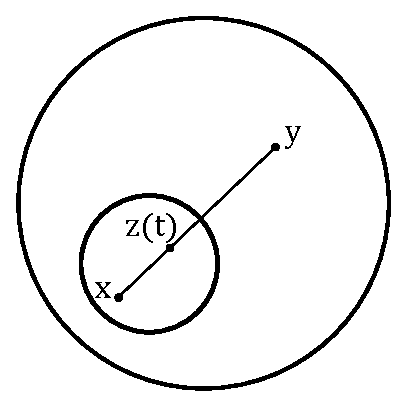
\includegraphics[scale=0.85]{images/6.eps} \\
	Следует заметить что $z(t) - x = t (y - x)$ т.е. при указанной гомотетии $y \to z(t)$, а якобиан преобразования очевидно равен $t^n$, так что
	\begin{equation*}
		\cdots = \int_{0}^{1}{\frac{dt}{t^n} \intset{\Omega(t)}{\left(u^\prime (z), \frac{z-x}{t}\right) dz}} = \int_{0}^{1}{\frac{dt}{t^{n+1}} \intset{\Omega(t)}{(u^\prime (z), z-x) dz}}  
	\end{equation*}
	далее перейдем к рассмотрению модуля разности
	\begin{multline*}
		\left|u(x) - \frac{1}{\mu(\Omega)} \intset{\Omega}{u(y)dy}\right| \leq 
		\mu(\Omega)^{-1} \int_{0}^{1}{\frac{dt}{t^{n+1}} \intset{\Omega(t)}{|(u^\prime (z), z-x)| dz}} \overset{\text{н-во К-Б-Ш}}{\leq} \\ \leq 
		\mu(\Omega)^{-1} \int_{0}^{1}{\frac{dt}{t^{n+1}} \intset{\Omega(t)}{|u^\prime (z)||z-x| dz}} \overset{\text{н-во Гельдера}}{\leq} \\ \leq 
		\mu(\Omega)^{-1} \int_{0}^{1}{\frac{dt}{t^{n+1}} \left(\intset{\Omega(t)}{|u^\prime (z)|^p dz}\right)^{\frac{1}{p}} \left(\intset{\Omega(t)}{|z-x|^{p^*} dz}\right)^{\frac{1}{p^*}} } \leq \\ \leq \mu(\Omega)^{-1} \norm{|u^\prime|}_{L^p (\Omega)} \int_{0}^{1}{\frac{dt}{t^{n+1}} \left(\intset{\Omega(t)}{|z-x|^{p^*} dz}\right)^{\frac{1}{p^*}}} = \cdots
	\end{multline*}
	\begin{multline*}
		\cdots = \mu(\Omega)^{-1} \norm{|u^\prime|}_{L^p (\Omega)} \int_{0}^{1}{\frac{dt}{t^{n+1}} \left(\intset{\Omega}{|t(y - x)|^{p^*} t^n dy}\right)^{\frac{1}{p^*}}} = \\ =
		\mu(\Omega)^{-1} \norm{|u^\prime|}_{L^p (\Omega)} \int_{0}^{1}{\frac{t\cdot t^{\frac{n}{p^*}}dt}{t^{n+1}} \left(\intset{\Omega}{|y - x|^{p^*} dy}\right)^{\frac{1}{p^*}}} \overset{|y-x| \leq \diam \Omega}{\leq} \\ \leq 
		\mu(\Omega)^{-1} \norm{|u^\prime|}_{L^p (\Omega)} \mu(\Omega)^{\frac{1}{p^*}} \diam \Omega \int_{0}^{1}{\frac{dt}{t^{n-\frac{n}{p^*}}}} = \\ =
		\mu(\Omega)^{-1 + \frac{1}{p^*}} \norm{|u^\prime|}_{L^p (\Omega)} \diam \Omega \left(\frac{t^{-\frac{n}{p} + 1}}{-\frac{n}{p} + 1} \bigg\rvert_0^1\right) = \frac{\diam \Omega}{1 - \frac{n}{p}} \norm{|u^\prime|}_{L^p (\Omega)} \mu(\Omega)^{-\frac{1}{p}}
	\end{multline*}
\end{proof}

\begin{lemma}{}{}\label{lemma:1}
	Пусть $u \in C^1 (\overline{B(0, 4R)})$, тогда для $\forall p > n \ \exists C = C(n, p, R)$ такое что
	\begin{equation*}
		\norm{u}_{C^{0, \bar{\alpha}}(\overline{B(0, R)})} \leq C \norm{u}_{1, p, B(0, 4R)}
	\end{equation*}
	, где $\bar{\alpha} = 1 - \frac{n}{p}$
\end{lemma}
\begin{proof}
	Введем обозначения $B_R = B(0, R)$ и $B_{4R} = B(0, 4R)$. \\ По определению
	\begin{equation*}
		\norm{u}_{C^{0, \bar{\alpha}} (\overline{B_R})} = \norm{u}_{C (\overline{B_R})} + [u]_{\bar{\alpha}, \overline{B_R}}
	\end{equation*}
	\textbf{1.} По предыдудыщей \hyperref[lemma:1]{лемме} получаем 
	\begin{equation*}
		\left| u(x) - \frac{1}{\mu(B_R)} \intset{B_R}{u(y) dy}  \right| \leq \underbrace{\frac{\overbrace{\diam B_R}^{2R}}{1 - \frac{n}{p}} \cdot \mu(B_R)^{-\frac{1}{p}}}_{C_0} \cdot \norm{|u^\prime|}_{L^p (B_R)}, \forall x \in \overline{B_R}
	\end{equation*}
	видим что $C_0 = C_0(n, p, R)$, используя обратное неравенство треугольника получаем
	\begin{multline*}
		|u(x)| \leq \frac{1}{\mu(B_R)} \intset{B_R}{|u(y)| dy} + C_0 \norm{ |u^\prime| }_{L^p (B_R)} \overset{\text{н-во Гельдера}}{\leq} \\ \leq \mu(B_R)^{-1} \left( \intset{B_R}{|u(y)|^p dy} \right)^{\frac{1}{p}} \left( \intset{B_R}{1^{p^*} dy} \right)^{\frac{1}{p^*}} + C_0 \norm{ |u^\prime|}_{L^p (B_R)} = \\ = \mu(B_R)^{\frac{1}{p}} \norm{u}_{L^p (B_R)} + C_0 \norm{ |u^\prime| }_{L^p (B_R)} \leq \cdots
	\end{multline*}
	теперь заметим что
	\begin{multline}\label{eq:2}
		\norm{ |u^\prime| }_{L^p (B_R)} = \left( \intset{B_R}{\left( \sqrt{\sum\limits_{i=1}^{n}{\left|\frac{\partial u}{\partial x_i}\right|^2}} \right)^{p} dx} \right)^{\frac{1}{p}} \leq \left( \intset{B_R}{\left( \sqrt{n} \sum\limits_{i=1}^{n}{\left| \frac{\partial u}{\partial x_i}\right|} \right)^{p} dx} \right)^{\frac{1}{p}} \leq \\ \leq
		n^{\frac{3}{2}} \left( \intset{B_R}{\left( \frac{1}{n} \sum\limits_{i=1}^{n}{\left| \frac{\partial u}{\partial x_i}\right|} \right)^{p} dx} \right)^{\frac{1}{p}} \leq n^{\frac{3}{2}} \left( \intset{B_R}{\frac{1}{n} \sum\limits_{i=1}^{n}{\left| \frac{\partial u}{\partial x_i}\right|^{p}} dx} \right)^{\frac{1}{p}} = n^{\frac{3}{2} - \frac{1}{p^*}} |u|_{1, p, B_R}
	\end{multline}
	итого т.к. $\alpha \norm{u}_{L^p (B_R)} + \beta |u|_{1, p, B_R} \leq 2 \max\{\alpha, \beta\} \norm{u}_{1, p, B_R}$, то
	\begin{equation*}
		\cdots \leq \mu(B_R)^{\frac{1}{p}} \norm{u}_{L^p (B_R)} + C_0 n^{\frac{3}{2} - \frac{1}{p^*}} |u|_{1, p, B_R} \leq C_1(n, p, R) \norm{u}_{1, p, B_R}
	\end{equation*}
	значит и 
	\begin{equation}\label{eq:3}
		\norm{u}_{C(\overline{B_R})} = \sup\limits_{x \in \overline{B_R}}{|u(x)|} \leq C_1 \norm{u}_{1, p, B_R}
	\end{equation} \\
	\textbf{2.} Пусть $\Omega = B\left(\frac{x_0 + y_0}{2}, \frac{|x_0 - y_0|}{2}\right)$ для $x_0, y_0 \in \overline{B_R}$. Пусть $x \in \Omega$, тогда
	\begin{equation*}
		|x| \leq \left|x - \frac{x_0 + y_0}{2}\right| + \left|\frac{x_0 + y_0}{2}\right| \leq \frac{|x_0 - y_0|}{2} + \frac{|x_0|}{2} + \frac{|y_0|}{2} < 2R
	\end{equation*}
	т.е. $x \in B(0, 2R)$, значит $\Omega \subset B_{2R}$ и $\overline{\Omega} \subset B_{4R}$. Очевидно $x_0, y_0 \in \overline{\Omega}$, заметим что
	\begin{multline*}
		|u(x_0) - u(y_0)| \leq \left|u(x_0) - \frac{1}{\mu(\Omega)} \intset{\Omega}{u(y) dy}\right| + \left| u(y_0) - \frac{1}{\mu(\Omega)} \intset{\Omega}{u(y) dy} \right| \leq \\ \leq 
		\frac{2 \diam \Omega}{1 - \frac{n}{p}} \cdot \mu(\Omega)^{-\frac{1}{p}} \cdot \norm{|u^\prime|}_{L^p (\Omega)} = \cdots
	\end{multline*}
	заметим что поскольку $\Omega$ это шар, то его диаметр это удвоенный радиус т.е. $\diam \Omega = |x_0 - y_0|$, а мера, как несложно показать с применением теоремы о геометрическом смысле интеграла Лебега пропорциональная $n$-ой степени диаметра т.е. $\mu(\Omega) = C_2 (n) |x_0 - y_0|^n$, так что
	\begin{equation*}
		\cdots = \frac{2 |x_0 - y_0|}{1 - \frac{n}{p}} \cdot C_2^{-\frac{1}{p}} (n) |x_0 - y_0|^{-\frac{n}{p}} \cdot \norm{|u^\prime|}_{L^p (\Omega)} \leq C_3 (n, p) |x_0 - y_0|^{1 - \frac{n}{p} = \bar{\alpha}} |u|_{1, p, B_{4R}}
	\end{equation*}
	последний переход выполнен при помощи \eqref{eq:2} с учетом $\Omega \subset B_{4R}$. Итого
	\begin{equation*}
		|u(x_0) - u(y_0)| \leq  C_3 |x_0 - y_0|^{\bar{\alpha}} |u|_{1, p, B_{4R}}, \forall x_0, y_0 \in \overline{B_R}
	\end{equation*}
	т.е. 
	\begin{equation}\label{eq:4}
		[u]_{\bar{\alpha}, \overline{B_R}} \leq [u]_{\bar{\alpha}, \overline{\Omega}} \leq C_3 (n, p) |u|_{1, p, B_{4R}}
	\end{equation}
	\textbf{3.} Объединив \eqref{eq:3} и \eqref{eq:4} получаем
	\begin{equation*}
		\norm{u}_{C^{0, \bar{\alpha} (\overline{B_R})}} \leq C_1 \norm{u}_{1, p, B_R} + C_3 |u|_{1, p, B_{4R}} \leq C_1 \norm{u}_{1, p, B_{4R}} + C_3 \norm{u}_{1, p, B_{4R}} \leq C \norm{u}_{1, p, B_{4R}}
	\end{equation*}
	где $C = C_1 (n, p, R) + C_3 (n, p) = C(n, p, R)$, ч.т.д.
\end{proof}

\begin{theorem}{2-ая теорема вложений Соболева}{}
	Пусть $\Omega$ -- липшицева ограниченная область, тогда
	\begin{equation*}
		p > n: W_p^1 (\Omega) \arrsubset C^{0, \alpha} (\overline{\Omega}), \forall \alpha \in [0, \bar{\alpha}]
	\end{equation*}
	, где $\bar{\alpha} = 1 - \frac{n}{p}$
\end{theorem}

\subsection{Случай компактных вложений}

\begin{theorem}{Реллиха, Кондрашова, Соболева}{}
	Пусть $\Omega \subset \Real^n$ -- липшицева ограниченная область, тогда
	\begin{enumerate}
		\item $p < n: W_p^1 (\Omega) \arrsubset\arrsubset L^q (\Omega), \forall q \in [0, \overline{p})$
		\item $p = n: W_p^1 (\Omega) \arrsubset\arrsubset L^q (\Omega), \forall q \in [0, +\infty)$
		\item $p > n: W_p^1 (\Omega) \arrsubset\arrsubset C^\alpha (\overline{\Omega}), \forall \alpha \in [0, \bar{\alpha})$
	\end{enumerate}
	, где $\overline{p} = \frac{np}{n-p}$ и $\bar{\alpha} = 1 -\frac{n}{p}$
\end{theorem}

\begin{lemma}{Теорема Реллиха}{}
	Пусть $\Omega \subset \Real^n$ -- липшицева ограниченная область, тогда
	\begin{equation*}
		W_p^1 (\Omega) \arrsubset\arrsubset L^p (\Omega)
	\end{equation*}
\end{lemma}

\begin{lemma}{}{}
	Пусть $\{u_k\}_{k\in\Natural} \subset L^q (\Omega)$ -- ограниченная последовательность, $1 < q < \infty$, причем $u_k \to u$ по мере в $\Omega$, тогда
	\begin{enumerate}
		\item $u \in L^q (\Omega)$
		\item $u_k \to u$ в $L^r (\Omega)$ для $1 \leq r < q$
	\end{enumerate}
\end{lemma}

\section{Граничный интеграл Лебега. Теория следов}

\subsection{Интеграл Лебега по поверхности}

Пусть $S \subset \Real^{n+1}$ определено как
\begin{equation*}
S = \{ (x^\prime, x_{n+1}) \in \Real^{n+1} \ | \ (x^\prime \in E) \wedge (x_{n+1} = \varphi(x^\prime))\}
\end{equation*}
где $\varphi \in C^1 (\overline{E})$, а $E$ -- ограниченная область в $\Real^n$. У $S$ нет $\mu_n$, а $\mu_{n+1} (S) = 0$. Попробуем ввести меру для $S$. Пусть $\Omega \subset S$ и 
\begin{equation*}
E_\Omega = \{ x^\prime \in E \ | \ (x^\prime, \varphi(x^\prime) \in \Omega)\} \subset \Real^n
\end{equation*}
Будем говорить что $\Omega$ измеримо в $S$ если $E_\Omega$ измеримо в $\Real^n$ и зададим меру:
\begin{equation*}
\mu_S (\Omega) = \intset{E_\Omega}{\sqrt{1 + \sum\limits_{i=1}^{n}{\frac{\partial \varphi}{\partial x_i} (x^\prime)}}dx^\prime}
\end{equation*}
Пусть $f : S \to \overline{\Real}$, введем несколько определений

\begin{definition}{Измеримая функция на поверхности}{}
	$f$ измерима на $S$ если $S[f \leq \alpha]$ -- измеримо в $S, \forall \alpha \in \Real$ 
\end{definition}

\begin{definition}{Суммируемость на поверхности}{}
	$f$ суммируема на $\Omega \subset S$ если
	\begin{equation*}
	\exists \intset{E_\Omega}{f(x^\prime, \varphi(x^\prime)) \sqrt{1 + \sum\limits_{i=1}^{n}{\frac{\partial \varphi}{\partial x_i} (x^\prime)}} dx^\prime}
	\end{equation*}
	который обозначают как 
	\begin{equation*}
	\intset{\Omega}{fdS}
	\end{equation*}
\end{definition}

Свойства интеграла Лебега переносятся, вводится пространство $L^p (S)$:
\begin{equation*}
\mathcal{L}^p (S) = \{ f : S \to \Real \ | \ |f|^p \text{ - суммируема на } S \}
\end{equation*}
и $L^p (S)$ -- факторпространство $\mathcal{L}^p (S)$ с нормой
\begin{equation*}
\norm{f}_{L^p (S)} = \left(\intset{S}{|f|^p dS}\right)^{\frac{1}{p}}
\end{equation*}

\subsection{Интеграл Лебега по границе области}

Пусть $\Omega$ -- ограниченная бласть в $\Real^n$, $\partial \Omega \in C^1$ (для $C^{0,1}$ с использованием \hyperref[th:2]{теоремы Радемахера} будет аналогично). Как следует из определения области класса $C^1$: $\forall x_0 \in \partial \Omega$
\begin{equation*}
	\exists R, L > 0 \ \exists \varphi \in C^{0, 1} (B^\prime) \ \exists Q_{x_0} \in \text{SO}(n)
\end{equation*}
такие что в системе координат $y = Q_{x_0} (x - x_0)$:
\begin{align*}
	B^\prime &= \{ y^\prime \in \Real^{n-1} \ | \ |y^\prime| < R \} \\
	C_{x_0} &= C_{R, 2RL} \\
	\partial \Omega \cap \overline{C_{x_0}} &= \{ y \in \Real^n \ | \ (|y^\prime| \leq R) \wedge (y_n = \varphi(y^\prime)) \} \\
	\Omega \cap \overline{C_{x_0}} &= \{ y \in \Real^n \ | \ (|y^\prime| \leq R) \wedge (-2RL < y_n < \varphi(y^\prime)) \}
\end{align*}
и поскольку $x_0 \in C_{x_0}$, то $\partial \Omega \subset \bigcup\limits_{x_0 \in \partial \Omega}{C_{x_0}}$, $\partial \Omega$ -- компакт, так что
\begin{equation*}
	\exists C_1 = C_{x_1}, ..., C_m = C_{x_m}: \ \partial \Omega \subset \bigcup\limits_{i=1}^{m}{C_m}
\end{equation*}
значит по \hyperref[th:3]{теореме о разбиении единицы} получаем что $\exists \psi_1, ..., \psi_m \in C^\infty (\Real^n)$:
\begin{enumerate}
	\item $0 \leq \psi_i \leq 1$
	\item $\supp \psi_i \ssubset C_i, \forall i \in \{1, ..., m\}$
	\item $\sum\limits_{i=1}^{m}{\psi_i} = 1$ на $\partial \Omega$
\end{enumerate}
Пусть теперь $\Gamma \subset \partial \Omega$ и $\Gamma_i = \Gamma \cap C_i$. Заметим что $\partial \Omega \cap C_i \subset \Real^n$ имеет вид
\begin{equation*}
	\partial \Omega \cap C_i = \{ (y^\prime, y_n) \in \Real^n \ | \ (y^\prime \in B_i^\prime) \wedge (y_n = \varphi_i (y^\prime)) \}
\end{equation*}
где $B_i^\prime = \{ y^\prime \in \Real^{n-1} \ | \ |y^\prime| < R_i \}$ и $R_i, \varphi_i$ получены из определения области класса $C^1$ для точки $x_i$. Определим $(B_i^\prime)_{\Gamma_i} = \{ y^\prime \in B_i^\prime \ | \ (y^\prime, \varphi_i (y^\prime)) \in \Gamma_i)\}$, тогда в терминах предыдущего параграфа можно определить все что нам нужно.

\begin{definition}{Измеримость на границе области}{}
	$\Gamma$ -- измеримо на $\partial \Omega$, если $(B_i^\prime)_{\Gamma_i}$ измеримо в $\Real^{n-1}$ для всякого $i \in \{1, ..., m\}$, причем задана мера
	\begin{equation*}
		\mu_{\partial \Omega}(\Gamma) = \sum\limits_{i=1}^{m}{\intset{\Gamma_i}{\psi_i d (\partial \Omega \cap C_i)}} = \sum\limits_{i=1}^{m}{\intset{(B_i^\prime)_{\Gamma_i}}{\psi_i (y^\prime, \varphi_i (y^\prime)) \sqrt{1 + \sum\limits_{k=1}^{n-1}{\frac{\partial \varphi_i}{\partial (y^\prime)_k} (y^\prime)}} dy^\prime} }
	\end{equation*}
\end{definition}
Функции $\psi_i$ нужны для того чтобы забить пересечения карт границы области. Пусть $f : \partial \Omega \to \overline{\Real}$

\begin{definition}{Измеримая функция на границе области}{}
	$f$ измерима на $\partial \Omega$ если $\partial \Omega [f \leq \alpha]$ -- измеримо на $\partial \Omega, \forall \alpha \in \Real$
\end{definition}

\begin{definition}{Суммируемость на границе области}{}
	$f$ суммируема на $\Gamma \subset \partial \Omega$ если
	\begin{equation*}
		\forall i \in \{1, ..., m\} \ \exists \intset{\Gamma_i}{f \psi_i d(\partial \Omega \cap C_i)}
	\end{equation*}
	тогда
	\begin{equation*}
		\intset{\Gamma}{f dS} = \sum\limits_{i=1}^{m}{\intset{\Gamma_i}{f \psi_i d(\partial \Omega \cap C_i)}}
	\end{equation*}
\end{definition}

Остается проверить что определения корректны, следующее утверждение устанавливает это
\begin{proposition}{}{}
	Определение меры на границе и интеграла по границе не зависит от покрытия цилиндрами и разбиения единицы.
\end{proposition}
Нетрудно заметить что $L^p (\partial \Omega)$ -- банаховы пространства, сепарабельные при $1 \leq p < \infty$ и рефлексивные при $1 < p < \Omega$, а $L^2 (\partial \Omega)$ -- гильбертово пространство.

\subsection{Оператор следа}

\begin{theorem}{}{}\label{th:4}
	Пусть $\Omega$ -- ограниченная область, $\partial \Omega \in C^{0, 1}$ и $1 \leq p < \infty$.  Тогда \\ $\exists C = C(n, p, \Omega)$:
	\begin{equation*}
		\norm{u}_{L^p (\partial \Omega)} \leq C \norm{u}_{1, p, \Omega}, \forall u \in C^1 (\overline{\Omega})
	\end{equation*}
\end{theorem}
Следствием этой теоремы является
\begin{proposition}{}{}
	Пусть выполнены условия \hyperref[th:4]{теоремы}, тогда $\forall \varepsilon > 0 \exists C = C(\varepsilon, n, p, \Omega)$:
	\begin{equation*}
		\norm{u}_{L^p (\partial \Omega)} \leq \varepsilon |u|_{1, p, \Omega} + C\norm{u}_{L^p (\Omega)}, \forall u \in C^1 (\overline{\Omega})
	\end{equation*}
\end{proposition}

Введя необходимые технические утверждения, можно приступить к определению оператора следа. Пусть $\partial \Omega \in C^{0, 1}$ и $\gamma_0: W_p^1 (\Omega) \to L^p (\partial \Omega)$ с областью определения $D(\gamma_0) = C^1 (\overline{\Omega})$. Сам оператор действует следующим образом
\begin{equation*}
	\gamma_0 u = u|_{\partial \Omega}
\end{equation*}
т.е. это оператор сужения, так что он линеен, к тому же ограничен по теореме из начала параграфа, а т.к. $C^\infty (\overline{\Omega}) \subset C^1 (\overline{\Omega})$, то по \hyperref[th:5]{теореме} -- $C^1 (\overline{\Omega}) = D(\gamma_0)$ всюду плотное в $W_p^1 (\Omega)$ множество и по теореме о продолжении оператора со всюду-плотной областью определения (применима ведь $L^p (\partial \Omega)$ банаховы) получаем

\begin{definition}{Оператор следа}{}
	Пусть $\Omega$ -- ограниченная липшицева область, оператором следа \\ $\gamma: W_p^1 (\Omega) \to L^p (\partial \Omega)$ называется продолжение оператора $\gamma_0$ на $W_p^1 (\Omega)$	
	Теперь мы можем ввести обозначение
	\begin{equation*} 
		u|_{\partial \Omega} = \gamma u, \forall u \in W_p^1 (\Omega)
	\end{equation*}
	это и есть след функции, причем для $u \in C^1 (\overline{\Omega})$ совпадает с определением сужения.
\end{definition}
\textbf{Замечание:} оператор следа устанавливает вложение $W_p^1 (\Omega) \arrsubset L^p (\partial \Omega)$, вложить подобным образом $L^p (\Omega)$ в $L^p (\partial \Omega)$ нельзя (!).

\begin{theorem}{}{}
	Для $1 < p < \infty$, $\gamma$ -- компактный оператор
\end{theorem}
Иначе говоря $W_p^1 (\Omega) \arrsubset\arrsubset L^p (\partial \Omega)$

\subsection{Свойства функций из пространств Соболева, связанные со следами}

\begin{theorem}{Интегрирование по частям}{}
	Пусть $u \in W_p^1 (\Omega)$, $v \in W_{p^*}^1 (\Omega)$, $\partial \Omega \in C^{0, 1}$, тогда
	\begin{equation*}
		\intset{\Omega}{u \frac{\partial_c v}{\partial x_i} dx} = \intset{\partial \Omega}{u|_{\partial \Omega} \cdot v|_{\partial \Omega} n_i dS} - \intset{\Omega}{v \frac{\partial_c u}{\partial x_i} dx}
	\end{equation*}
	где $n_i$ -- $i$-ая координата нормали $n$ к $\partial \Omega$.
\end{theorem}

\begin{theorem}{Теорема о склейке}{}
	Пусть $\Omega_1 \cap \Omega_2 = \emptyset$, $\partial \Omega_1 \in C^{0, 1}, \partial \Omega_2 \in C^{0, 1}$ и $\Omega = \Omega_1 \cup \Omega_2$ (склейка непересекающихся областей). Пусть $\Gamma = \partial \Omega_1 \cap \partial \Omega_2$ (общая граница по которой склеили). Если $u \in W_p^1 (\Omega_1), \\ u \in W_p^1 (\Omega_2)$ и $\mu_{\partial \Omega_1} (\Gamma) = \mu_{\partial \Omega_2} (\Gamma) \neq 0$, то для функции 
	$u = 
	\begin{cases}
		u_1 \text{ в } \Omega_1  \\
		u_2 \text{ в } \Omega_2  
	\end{cases}$ справедливо
	\begin{equation*}
		\left( u \in W_p^1 (\Omega) \right) \Leftrightarrow \left( u_1|_\Gamma = u_2|_\Gamma \right)
	\end{equation*}
	(след этих функций на общей границе должен совпадать)
\end{theorem}

\begin{theorem}{}{}
	Пусть $\partial \Omega \in C^{0, 1}$, тогда
	\begin{equation*}
		\mathring{W_p^1} (\Omega) = \{ u \in W_p^1 (\Omega) \ | \ u|_{\partial \Omega} = 0\}
	\end{equation*}
\end{theorem}

\newpage

\tcblistof[\section*]{def}{Список определений}

\end{document}
